\chapter{Schroedinger equation in 1d}
%
In this chapter we will be concentrating on the problem of
finding bound states solution to time-independent
Schroedinger equation in one dimension:
\begin{equation}
\left[ -\frac{1}{2}\frac{\mathrm{d}^2}{\mathrm{d}x^2} + V(x) \right] \psi(x) = E\, \psi(x)
\label{eq:Sch_1d_eq}
\end{equation}
%
with the boundary conditions:
%
\begin{equation}
\lim_{x \rightarrow \pm \infty} \psi(x) = 0
\label{eq:BC_isolated}
\end{equation}
%
This boundary condition is relevant for non-periodic systems such as
isolated or free atoms and molecules.

\section{Grid points}

We need to define a spatial domain $\left[x_{\mathrm{min}}, x_{\mathrm{max}}\right]$
where $x_{\mathrm{min}}, x_{\mathrm{max}}$ chosen
such that the boundary condition \ref{eq:BC_isolated} is approximately satisfied.
The next step is to divide the spatial domain $x$ using equally-spaced grid points
which we will denote as $\{x_{1},x_{2},\ldots,x_{N}\}$ where $N$ is total number
of grid points. Various spatial quantities such as wave function $\psi(x)$
and potential $\psi(x)$ will be discretized on these grid points.

The grid points $x_{i}$, $i = 1, 2, \ldots$ are chosen to be:
%
\begin{equation}
x_{i} = x_{\mathrm{min}} + (i-1)h
\end{equation}
%
where $h$ is the spacing between the grid points:
%
\begin{equation}
h = \frac{ x_{\mathrm{max}} - x_{\mathrm{min}} }{N-1}
\end{equation}

The following Julia function can be used to initialize the grid points.
\begin{juliacode}
function init_FD1d_grid( x_min::Float64, x_max::Float64, N::Int64 )
  L = x_max - x_min
  h = L/(N-1) # spacing
  x = zeros(Float64,N) # the grid points
  for i = 1:N
    x[i] = x_min + (i-1)*h
  end
  return x, h
end
\end{juliacode}
The function \jlinline{init_FD1d_grid} takes three arguments:
\begin{itemize}
\item \jlinline{x_min::Int64}: the left boundary point
\item \jlinline{x_max::Int64}: the right boundary point
\item \jlinline{N::Float64}: number of grid points
\end{itemize}
The function will return $x$ which is an array of grid points and $h$ which
is the uniform spacing between grid points. The boundary points \jlinline{x_min}
and \jlinline{x_max} will be included in the grid points.

As an example of the usage of the function \jlinline{init_FD1d_grid}, let's
sample and plot a Gaussian function
%
\begin{equation}
\psi(x) = \mathrm{e}^{-\alpha x^2}
\label{eq:gauss_func1}
\end{equation}
%
where $\alpha$ is a positive number. We will sample the function
within the domain $[x_{\text{min}},x_{\text{max}}]$ where
$x_{\text{min}}=-5$ and $x_{\text{max}}=5$.
The Gaussian function defined in \eqref{eq:gauss_func1} can be implemented
as the following function.
\begin{juliacode}
function my_gaussian(x::Float64; α=1.0)
  return exp( -α*x^2 )
end
\end{juliacode}
Note that we have set the default value of parameter $\alpha$ to 1.

The full Julia program is as follows.
%
\begin{juliacode}
using Printf
using LaTeXStrings

import PyPlot
const plt = PyPlot
plt.rc("text", usetex=true)

include("init_FD1d_grid.jl")

function my_gaussian(x::Float64; α=1.0)
  return exp( -α*x^2 )
end

function main()
  A = -5.0
  B =  5.0
  Npoints = 8
  x, h = init_FD1d_grid( A, B, Npoints )
  @printf("Grid spacing = %f\n", h)
  @printf("\nGrid points:\n")
  for i in 1:Npoints
    @printf("%3d %18.10f\n", i, x[i])
  end
  NptsPlot = 200
  x_dense = range(A, stop=5, length=NptsPlot)
  plt.clf()
  plt.plot(x_dense, my_gaussian.(x_dense), label=L"f(x)")
  plt.plot(x, my_gaussian.(x), label=L"Sampled $f(x)$", marker="o")
  plt.legend()
  plt.tight_layout()
  plt.savefig("IMG_gaussian_1d_8pt.pdf")
end
main()
\end{juliacode}

After execution, the program will print grid spacing and grid points to the standard
output and also plot the function to a file named \jlinline{IMG_gaussian_1d_8pt.pdf}
You may try to experiment by changing the value of \jlinline{N} and compare the result.
The resulting plots for \jlinline{N=8} and \jlinline{N=21} are shown in Figure XXX.
\begin{figure}[H]
{\center
\includegraphics[width=0.65\textwidth]{../codes/FD1d/IMG_gaussian_1d_8pt.pdf}
\includegraphics[width=0.65\textwidth]{../codes/FD1d/IMG_gaussian_1d_21pt.pdf}
\par}
\caption{Sampling a Gaussian function}
\end{figure}


\section{Approximating second derivative operator}

Our next task is to find an approximation to the second derivative operator
present in the Equation \eqref{eq:Sch_1d_eq}.
One simple approximation that we can use is the 3-point (central) finite difference:
\begin{equation}
\frac{\mathrm{d}^2}{\mathrm{d}x^2} \psi_{i} =
\frac{\psi_{i+1} - 2\psi_{i} + \psi_{i-1}}{h^2}
\end{equation}
where we have the following notation have been used: $\psi_{i} = \psi(x_{i})$.
%
By taking $\{ \psi_{i} \}$ as a column vector, the second derivative operation
can be expressed as matrix multiplication:
\begin{equation}
\vec{\psi''} \approx \mathbb{D}^{(2)} \vec{\psi}
\end{equation}
%%
where $\mathbb{D}^{(2)}$ is the second derivative matrix operator:
%
\begin{equation}
\mathbb{D}^{(2)} = \frac{1}{h^2}
\begin{bmatrix}
-2  &  1  &  0  &  0  & 0 & \cdots & 0 \\
 1  & -2  &  1  &  0  & 0 & \cdots & 0 \\
 0  &  1  & -2  &  1  & 0 & \cdots & 0 \\
 \vdots  &  \ddots  &  \ddots  & \ddots  & \ddots  & \ddots & \vdots \\
 0 & \cdots & 0 & 1 & -2 & 1 & 0 \\
 0  &  \cdots  & \cdots & 0  & 1  & -2  & 1 \\
 0  &  \cdots  & \cdots & \cdots & 0  &  1  & -2 \\
\end{bmatrix}
\label{eq:1d_D2_matmul}
\end{equation}

An example implementation can be found in the following function.
\begin{juliacode}
function build_D2_matrix_3pt( N::Int64, h::Float64 )
  mat = zeros(Float64,N,N)1
  for i = 1:N-1
    mat[i,i] = -2.0
    mat[i,i+1] = 1.0
    mat[i+1,i] = mat[i,i+1]
  end
  mat[N,N] = -2.0
  return mat/h^2
end
\end{juliacode}
The function \jlinline{build_D2_matrix_3pt} takes two arguments:
\begin{itemize}
\item \jlinline{N::Int64}: number of grid points
\item \jlinline{h::Float64}: the uniform grid spacing
\end{itemize}

Before use these functions to solve Schroedinger equation, we will test the operation
in Equation \eqref{eq:1d_D2_matmul} for a simple function for which the second derivative
can be calculated analytically. This function also should satisfy the boundary condition
\ref{eq:BC_isolated}. We will take the the Gaussian function
\eqref{eq:gauss_func1} that we have used before.
The second derivative of this Gaussian function can be calculated as
%
\begin{equation}
\psi''(x) = \left( -2 \alpha + 4\alpha^2 x^2 \right) \mathrm{e}^{-\alpha x^2}
\end{equation}

We also need to define the computational domain $[A,B]$ for our test.
Let's choose $A = -5$ and $B = 5$ again as in the previous example.
We can evaluate the value of function $\psi_{x}$ at those points to be at the
order of $10^{-11}$, which is sufficiently small for our purpose.

The full Julia script that we will use is as follows.
\begin{juliacode}
using Printf
using LaTeXStrings

import PyPlot
const plt = PyPlot
plt.rc("text", usetex=true)

include("init_FD1d_grid.jl")

function my_gaussian(x::Float64; α=1.0)
  return exp( -α*x^2 )
end

function main()
  A = -5.0
  B =  5.0
  Npoints = 8
  x, h = init_FD1d_grid( A, B, Npoints )
  @printf("Grid spacing = %f\n", h)
  @printf("\nGrid points:\n")
  for i in 1:Npoints
    @printf("%3d %18.10f\n", i, x[i])
  end

  NptsPlot = 200
  x_dense = range(A, stop=5, length=NptsPlot)

  plt.clf()
  plt.plot(x_dense, my_gaussian.(x_dense), label=L"f(x)")
  plt.plot(x, my_gaussian.(x), label=L"Sampled $f(x)$", marker="o")
  plt.legend()
  plt.tight_layout()
  plt.savefig("IMG_gaussian_1d.pdf")
end

main()
\end{juliacode}

\begin{figure}[H]
{\center
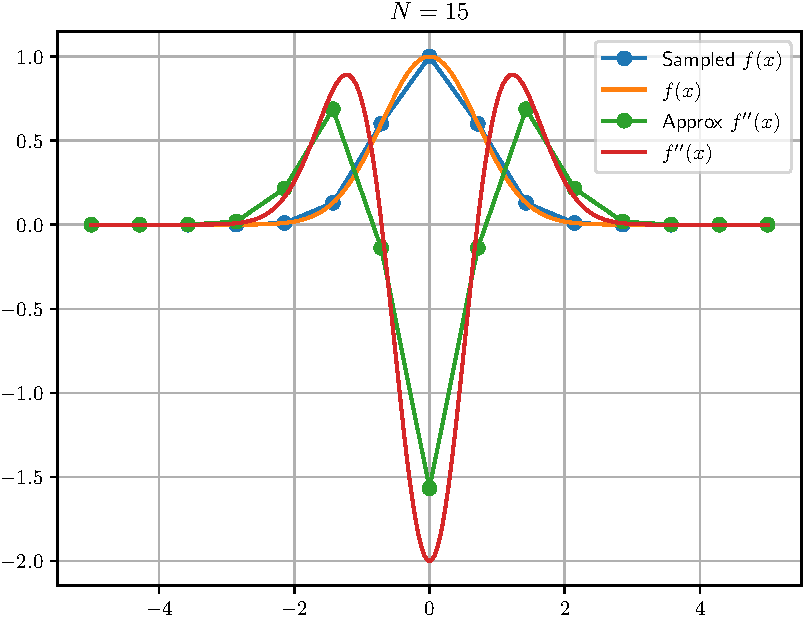
\includegraphics[width=0.65\textwidth]{../codes/FD1d/IMG_gaussian_15.pdf}
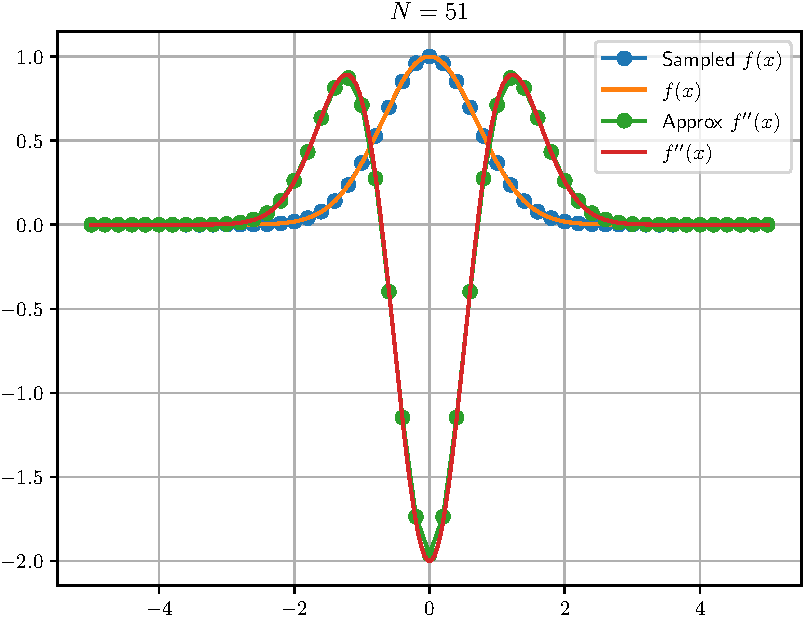
\includegraphics[width=0.65\textwidth]{../codes/FD1d/IMG_gaussian_51.pdf}
\par}
\caption{Finite difference approximation to a Gaussian function and its second derivative}
\end{figure}


\section{Harmonic potential}

We will start with a simple potential with known exact solution, namely the harmonic potential:
\begin{equation}
V(x) = \frac{1}{2}\omega^2 x^2
\end{equation}

The Hamiltonian in finite difference representation:
\begin{equation}
\mathbb{H} = -\frac{1}{2}\mathbb{D}^{(2)} + \mathbb{V}
\end{equation}
where $\mathbb{V}$ is a diagonal matrix whose elements are:
\begin{equation}
\mathbb{V}_{ij} = V(x_{i})\delta_{ij}
\end{equation}


Code to solve harmonic oscillator:

\juliafile{../codes/sch_1d/main_harmonic_01.jl}

Compare with analytical solution.

Plot of eigenfunctions:

\begin{figure}[H]
{\center
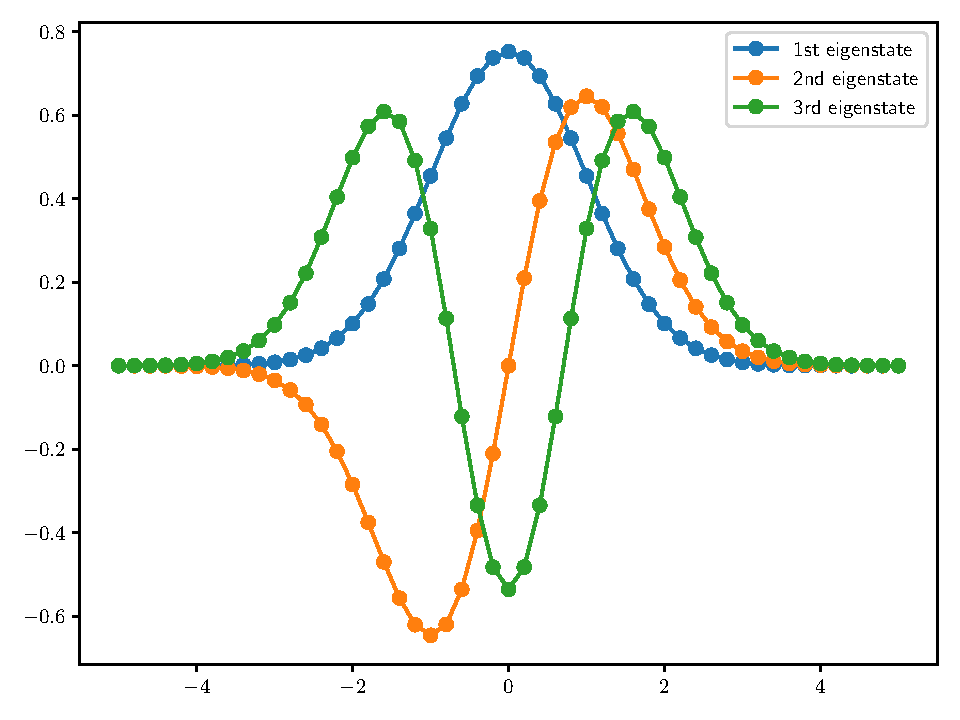
\includegraphics[scale=0.75]{../codes/sch_1d/IMG_main_harmonic_01_51.pdf}
\par}
\caption{Eigenstates of harmonic oscillator}
\end{figure}


\section{Higher order finite difference}

To obtain higher accuracy

Implementing higher order finite difference.


\section{Exercises}

Gaussian potential
